% !TeX root = main.tex
% !TeX encoding = UTF-8
% !TeX spellcheck = <none>
%% Chapter03-机载LiDAR数据获取基本原理.tex

\chapter{机载LiDAR数据获取基本原理} %% Chapter 机载LiDAR数据获取基本原理

\section{数据获取重要参数}  %% Section	数据获取重要参数	========================================
\subsection{LiDAR数据获取重要参数的作用}
\begin{itemize}
	\item 与LiDAR系统性能、数据质量相关的参数关系式或计算公式。
	\item 是进行激光遥感系统选择及航线设计的重要依据!
\end{itemize}

\subsection{参数类型}

%p
\kaiparagraph{瞬时视场角(instantaneous field of view, IFOV)} 又称\textit{激光发散角},是指激光束发射时其发散的角度。瞬时视场角的大小取决于激光的衍射(diffraction),是发射孔径$ D $和激光波长$ λ $的函数:
\begin{equation}
\text{IFOV} = 2.44 \dfrac{\lambda}{D}
\end{equation}

%p
\kaiparagraph{视场角(Field Of View, FOV)} 激光束的扫描角,指激光束通过扫描装置所能达到的最大角度范围。

早期LiDAR系统的扫描角一般较小,大约在$ 30^{\circ} $,目前比较先进的LiDAR系统的扫描角都在$ 60^{\circ} \sim 75^{\circ} $度左右,基本能够达到航摄像机的视场角度范围。

%p
\kaiparagraph{脉冲频率}单位时间内激光器所能够发射的激光束数量。

\textbf{注意}:并不是脉冲频率越大越好,过于密集的激光脚点会带来大量的冗余数据,影响数据处理的效率和效果。

%p
\kaiparagraph{扫描频率} 扫描频率指线扫描方式,每秒钟所扫描的行数,即扫描镜每秒钟摆动的周期。很明显,扫描频率越大,每秒钟的扫描线就越多。

%p
\kaiparagraph{垂直分辨率}脉冲通过的路径上所能够区分不同目标间的最小距离。
\begin{equation}
H_{\min} = c \dfrac{t_{\min}}{2}
\end{equation}
若脉冲宽度为10 ns,则在一个脉冲宽度内,不同目标距离至少为1.5 m,其回波能量才可能经接收器检出,并区别开来。

%p
\kaiparagraph{最大飞行高度(最大量测距离)}系统所能精确测定的最远距离。

在实际中工程中,其影响因素有很多:激光功率、光束的发散性、大气折射率、地物反射率、探测器灵敏度等等。

%p
\kaiparagraph{最小飞行高度}取决于
\begin{itemize*}
	\item 飞行平台的类型
	\item 探测地区的地形
	\item 人眼的安全距离
\end{itemize*}

%p
\kaiparagraph{激光脚点光斑特性}包含三个方面:
\begin{enumerate}
	\item \textit{激光脚点光斑直径(激光束照射面直径)}:
		地面上瞬时激光脚点投射在地面上为一个椭圆形的光斑,其航向直径(航线方向,短轴)与旁向直径(扫描方向,长轴)是不等的;
		它们与下列因素有关:平台的飞行高度$ H $;激光波束发散角$ γ $;地形坡度$ α $;瞬时扫描角$ θ_i $。关系如图所示。
		
		\begin{figure}[htbp]
			\centering
			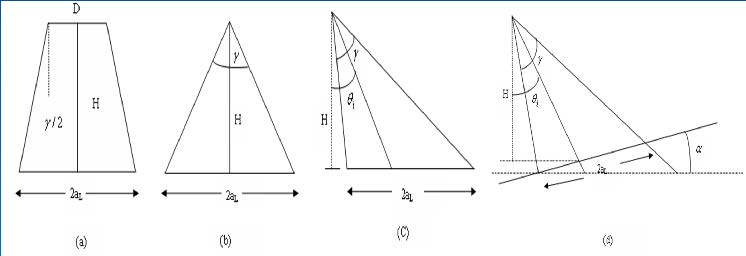
\includegraphics[width=0.8\linewidth]{figure/Chapter4/激光脚点直径}
			\caption{激光脚点直径}
			\label{fig:激光脚点直径}
		\end{figure}
		
		\begin{enumerate}
			\item 当遥感平台处于水平状态,激光束垂直照射水平地面上(瞬时扫描角$ θ_i=0 $)时(图\ref{fig:激光脚点直径}-a),激光脚点光斑的旁向直径
				\begin{equation}
				2a_L = D + 2H \tan \dfrac{\gamma}{2}
				\end{equation}
				通常探测器孔径$ D $比较小,只有10$ \sim $15 cm,可以忽略(图\ref{fig:激光脚点直径}-b)。故有:
				\begin{equation}
				2a_L \approx 2H \tan \dfrac{\gamma}{2}
				\end{equation}
				由于激光波束发散角$ γ $也非常小,可简化为:
				\begin{equation}
				2a_L \approx 2H \dfrac{\gamma}{2} \approx H \gamma
				\end{equation}
			\item 当遥感平台处于水平状态,激光束倾斜(瞬时扫描角为$ θ_i $)照射水平地面上时(图\ref{fig:激光脚点直径}-c),旁向直径:
				\begin{equation}
				2a_L = H \tan\left( \theta_i + \dfrac{\gamma}{2}\right)  - H \tan\left(\theta_i - \dfrac{\gamma}{2}\right)
				\end{equation}
			\item 当遥感平台处于水平状态,激光束倾斜(瞬时扫描 角为$ θ_i $),照射到倾斜地面(坡度为$ α $)上时(图\ref{fig:激光脚点直径}-d),激光脚点光斑的旁向直径
				\begin{equation}
				2a_L = \dfrac{H\sin\dfrac{\gamma}{2}}{\cos \theta_i \cos \left(\theta_i + \dfrac{\gamma}{2} - \alpha \right)}
				     + \dfrac{H\sin\dfrac{\gamma}{2}}{\cos \theta_i \cos \left(\theta_i - \dfrac{\gamma}{2} - \alpha \right)}
				\end{equation}
			\item 对于激光脚点的航向直径,始终为
				\begin{equation}
				2a_L \approx H \gamma
				\end{equation}
		\end{enumerate} % 激光脚点光斑直径(激光束照射面直径)
	\item \textit{回波多值性}:由于激光脚点在地面形成光斑,具有一定的面积。在此区域内也许存在不同的地物类型或者地面有起伏。这些都会造成同一束激光脉冲可能有多个回波信号。这些信号可能先后到达接收器,就形成多次回波。
		\begin{figure}[htbp]
			\centering
			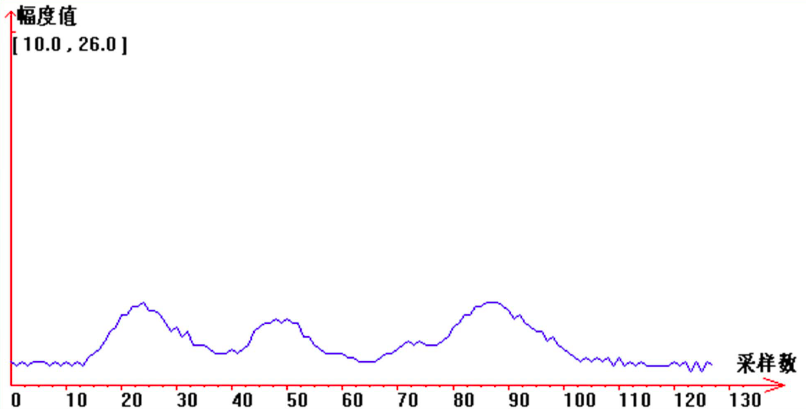
\includegraphics[width=0.5\linewidth]{figure/Chapter4/回波多值性}
			\caption{回波多值性}
			\label{fig:回波多值性}
		\end{figure}
	\item \textit{动态重合系数$ Q $}:激光脚点光斑与接收脚印
		\footnote{由于遥感平台的移动的关系,在反射光束到达接收装置的时候,已经不是原来的激光脚点的位置、大小和形状了,形成接收脚印。由于平台的移动,接收脚印与激光脚点光斑通常只有部分重合。}
		重合部分的面积与激光光斑的面积之比。
		
		\textbf{影响因素}:\begin{itemize*}
			\item 激光波束发散角
			\item 接收瞬时视场角
			\item 传感器平台高度
			\item 扫描镜速度
			\item 波束倾角
		\end{itemize*}
\end{enumerate} % 激光脚点光斑特性

\kaiparagraph{扫描带宽SW}一般来说,激光束扫描角即激光扫描视场角是一个已知量, 在确定飞行高度的情况下,可以计算出扫描带宽:
\begin{equation}
\symrm{SW} = 2H \tan \dfrac{\theta}{2}
\end{equation}
\begin{itemize}
	\item 对于椭圆扫描工作方式仍适用,因为扫描角的量度以天底点方向为准。
	\item 对于Z形扫描,实际扫描宽度长一些。
\end{itemize}

\kaiparagraph{扫描行的点数$ N $}在扫描视场角的范围内可以发射多少束激光,即一扫描行内扫描点的数量。该参数关系到扫描量测点的密度。

根据脉冲重复频率\footnote{每秒钟发射激光脉冲的次数}$ F $和扫描频率\footnote{每秒钟扫描行数}$ f_{sc} $,可计算每一扫描行的点数:
\begin{equation}
N = \dfrac{F}{f_{sc}}
\end{equation}

\textbf{注意}:可见,$ N $与飞行高度和扫描带宽无关。扫描点数计算与飞行高度、扫描带宽无关!
由于不同的区域所需的量测密度不同,当激光扫描仪的扫描频率和脉冲重复频率固定时,即一行扫描点的个数固定;若此时针对具体区域制订飞行计划,要求点的密度要大一些,就要考虑适当降低飞行高度。

\kaiparagraph{激光脚点间距(Point Space)}如图\ref{fig:激光脚点间距}所示,分为航向脚点间距和旁向脚点间距。
\begin{figure}[htbp]
	\centering
	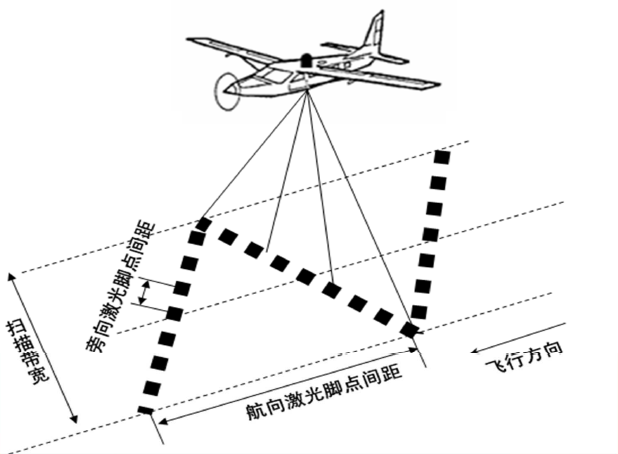
\includegraphics[width=0.5\linewidth]{figure/Chapter4/激光脚点间距}
	\caption{激光脚点间距}
	\label{fig:激光脚点间距}
\end{figure}

\begin{enumerate}
	\item \textit{航向脚点间距$ \diff x_{\text{along}} $}:沿飞行方向扫描点之间的距离称为航向点距。
		\begin{itemize}
			\item \textbf{一般扫描方式}:
				根据飞机飞行速度$ v $,计算得到点距
				\begin{equation}
				\diff x_{\text{along}} = \dfrac{v}{f_{sc}}
				\end{equation}
				式中,$ v $为飞行速度,$ f_{sc} $为扫描频率。可见,航向激光脚点间距也与飞行高度无关,只与飞行速度和扫描频率有关。
			\item \textbf{椭圆扫描方式}:飞行方向上点距较大。
			\item \textbf{Z形扫描方式}:由于有两种定义扫描行的方式,计算飞行方向点距也有两种方式。如图\ref{fig:Z形扫描的激光脚点间距}所示。
				\begin{figure}[htbp]
					\centering
					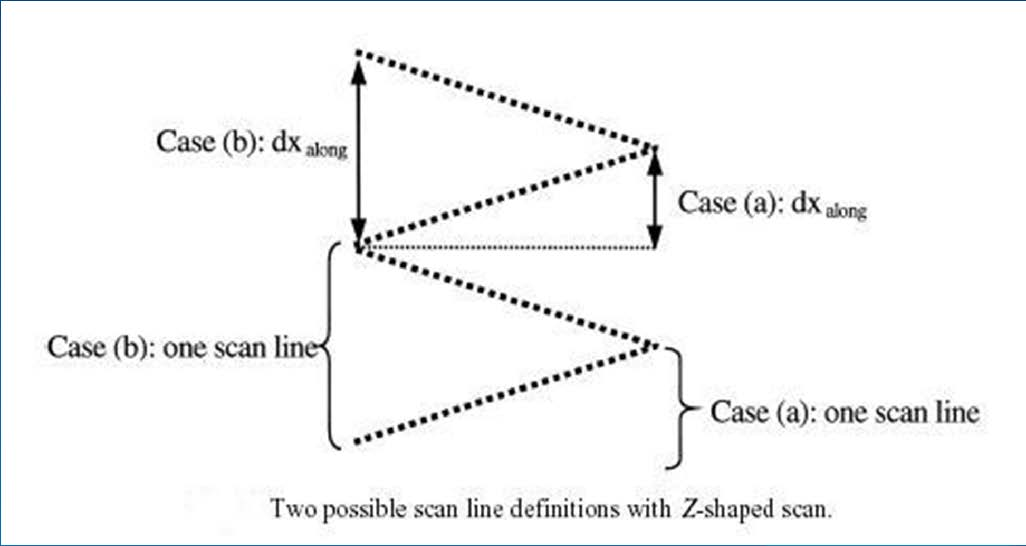
\includegraphics[width=0.5\linewidth]{figure/Chapter4/Z形扫描的激光脚点间距}
					\caption{Z形扫描的激光脚点间距}
					\label{fig:Z形扫描的激光脚点间距}
				\end{figure}
		\end{itemize} % 航向脚点间距
	\item \textit{旁向脚点间距$ \diff x_{\text{across}} $}:旁向激光脚点间距指一条扫描线上相邻激光脚点的间距,旁向激光脚点间距与扫描带宽SW和每条扫描点上的激光脚点数$ N $相关。
		\begin{itemize}
			\item \textbf{一般扫描方式}:
				\begin{equation}
				\diff x_{\text{across}} = \dfrac{\symrm{SW}}{N}
				\end{equation}
			\item \textbf{光纤扫描}:
				\begin{equation}
				\diff x_{\text{across}} = h \dfrac{\theta}{N-1}
				\end{equation}
			\item \textbf{椭圆扫描}:在接近圆形扫描的情况下,扫描方向点距可按下式作近似估计:
				\begin{equation}
				\diff x_{\text{across}} = \pi \dfrac{\symrm{SW}}{N}
				\end{equation}
				椭圆扫描是由旋转棱镜实现的,根据其镜面和转轴垂面之间的夹角SN,可以较精确地计算扫描方向点距:
				\begin{equation}
				\diff x_{\text{across}} = \dfrac{4.4429 h}{N} \sqrt{\tan^2 \left(2\symrm{SN}\right) + \tan^2 \left(1.41\symrm{SN}\right)}
				\end{equation}
		\end{itemize} % 旁向脚点间距
\end{enumerate} % 激光脚点间距

\kaiparagraph{最少航带数}对于需要进行激光量测的区域,在执行量测任务之前,应对飞行航带数进行估计,若其宽度为$ W $ km ,航带之间扫描重叠度为$ q $。所需航带数为
\begin{equation}
n = \min n_i
\end{equation}
满足
\begin{equation}
(n_i - 1) \geqslant \dfrac{W - \symrm{SW}}{\symrm{SW}(1-q)}
\end{equation}
即
\begin{equation}
n = \symrm{int} \left[ \dfrac{W - \symrm{SW}}{\symrm{SW}(1-q)} + 1\right]
\end{equation}

\textbf{意义}:扫描带宽是一个重要参量,要计算扫描带宽,又与航高有关,
在实际制定飞行计划时,航高的确定须根据区域内的最低点,而航带重叠度的计算则要依据区域内最高点,以避免在扫描带宽很窄的情况下产生遗漏。

\kaiparagraph{实际量测面积}在估算出所需航带数的基础上,可以对激光扫描量测的实际覆盖区域面积进行计算。如果飞机速度为$ v $,待量测区域长度为$ L $,那么,实际量测面积为
\begin{align}
\begin{split}
A & = \symrm{SW} v T_S [(n - 1)(1 - q) + 1] \\
& = \symrm{SW} L [(n - 1)(1 - q) + 1]
\end{split}
\end{align}

\kaiparagraph{量测点密度}计算出实际量测面积后,实际量测点密度按下式计算:
\begin{equation}
d = \dfrac{FnT_S}{A}
\end{equation}

\kaiparagraph{量测点数据量}实际量测点数据量涉及到数据存储空间的问题,如果需要在飞机上实时计算出地面每一被量测点的三维坐标,并记录下每一个点的反射强度,
每点序号、坐标$ (X,Y,Z) $和时间按4字节记录,强度按一个字节记录,每点需要21个字节,数据总量为
\begin{equation}
C = FT_f \times 21 \text{bytes}
\end{equation}
式中,$ T_f $是激光扫描量测所需的全部时间。

\kaiparagraph{发射及接收激光束间隔内的飞行距离}在激光器发射脉冲到接收地面发射的脉冲有一个时间间隔,在此间隔内一个平台移动了一段距离
\begin{equation}
d = v \times \diff t = \dfrac{2vR}{c}
\end{equation}
一般而言,在以飞机为平台时,这段距离很短。这影响到动态重合系数的大小。

\kaiparagraph{过采样和欠采样}沿扫描方向的估计式为
\begin{equation}
Q_{\text{across}} = \dfrac{2a_L}{\diff x_{\text{across}}}
\end{equation}
如果$ Q_{\text{across}} > 1$,就是过采样,反之就是欠采样。

\section{常用商业LiDAR系统}
\paragraph{Leica公司LiDAR设备}
\paragraph{Optech公司LiDAR设备}
\paragraph{Riegl公司LiDAR设备}